\documentclass[11pt, reqno]{elsarticle}%
\usepackage{lipsum}
\makeatletter
\def\ps@pprintTitle{%
 \let\@oddhead\@empty
 \let\@evenhead\@empty
 \def\@oddfoot{}%
 \let\@evenfoot\@oddfoot}
\makeatother


%\documentclass[journal]{IEEEtran}

\usepackage{amsmath}
\usepackage{tikz}
\usetikzlibrary{arrows.meta}

\usepackage{bbm}
\interdisplaylinepenalty=2500

%\usepackage[dvipsnames]{xcolor}
\usepackage{array}
\usepackage{amssymb}
\usepackage{amsthm}
\theoremstyle{plain}

\usepackage{dsfont} %for characterisic function (\mathds{1})

\usepackage[margin=1in]{geometry}
%\usepackage{graphicx}
%\usepackage{subfigure}                                     
\usepackage[bookmarks=false]{hyperref}
\usepackage{cleveref}
\usepackage{epstopdf}

\def\xx{{\bf x}}
\def\ww{{\bf w}}
\def\yy{{\bf y}}
\def\uu{{\bf u}}
\def\vv{{\bf v}}
\def\+{{\oplus}}
\newcommand{\p}{\mathbb{P}}
\newcommand{\Ff}{{\mathbb F}}
\newcommand{\Zz}{{\mathbb Z}}
\newcommand{\Cc}{{\mathbb C}}
\newcommand{\Qq}{{\mathbb Q}}
\newcommand{\R}{{\mathcal R}}
\newcommand{\Ll}{{\mathcal L}}
\newcommand{\Fl}{{\mathcal F}}
\newcommand{\bv}{{\bf v}}
\newcommand{\bw}{{\bf w}}
\newcommand{\cP}{{\mathcal P}}
\newcommand{\cB}{{\mathcal B}}
\newcommand{\cD}{{\mathcal D}}
\newcommand{\Trace}{{\rm Tr}}
\newcommand\im{\operatorname{Im}}
\newcommand\Ker{\operatorname{Ker}}
\newcommand\Order{\operatorname{Ord}}
\newcommand\MM{{\overline M}}
\newcommand\MN{{\overline N}}
\newcommand\pp{{\mathfrak p}}
\newcommand\bbar{{\overline{\Cal B}}}
\newcommand\cc{{\mathcal C}}
\newcommand\llambda{{\pmb\lambda}}
\newcommand{\gf}{ {{\mathbb F}} }
\newcommand{\image}{{\rm Image}}
\newcommand{\aut}{{\rm Aut}}

\newcommand{\pa}{p_i^{\uparrow}}
\newcommand{\pd}{p_i^{\downarrow}}

\newcommand{\rme}{\mathrm{e}}
\newcommand{\rmd}{\mathrm{d}}
\newcommand{\rmi}{\mathrm{i}}

\newcommand{\new}[2]{{\color{Red}#2}}
\newcommand{\takeout}[1]{{\color{Orange}#1}}
\newcommand{\drop}[1]{{\color{Orange}\textbf{DROP}[#1]}}

\def\Tr{\operatorname{Tr}}
\def\tr{\operatorname{tr}}
\def\Im{\operatorname{Im}}
\def\PG{\operatorname{PG}}
\def\Sp{\operatorname{Sp}}
\def\dmid{\,||\,}
\newtheorem*{theorem*}{Theorem}
\newtheorem{thm}{Theorem}%[section]
\newtheorem{theorem}[thm]{Theorem}%[section]
%\newtheorem{proof1}{Proof}[subsection]
\newtheorem{lemma}[thm]{Lemma}
\newtheorem{cor}[thm]{Corollary}
\newtheorem{conj}[thm]{Conjecture}
\newtheorem{prop}[thm]{Proposition}
\newtheorem{prob}[thm]{Problem}
%\newtheorem{proof}[thm]{Proof}
\newtheorem{defn}[thm]{Definition}
\newtheorem{example}[thm]{Example}
\newtheorem{remark}[thm]{Remark}
\def\Tr{\operatorname{Tr}}
\def\tr{\operatorname{tr}}
%\numberwithin{equation}{section}

\setlength\parindent{0pt} %to have no indent


\newcounter{comments}
 
\newcommand{\sai}[1]{\addtocounter{comments}{1}{\color{red}[Sai \thecomments: #1]}}
\newcommand{\ck}[1]{\addtocounter{comments}{1}{\color{blue}[Claus \thecomments: #1]}}
\newcommand{\mw}[1]{\addtocounter{comments}{1}{\color{orange}[Matt \thecomments: #1]}}
\newcommand{\todo}[1]{\addtocounter{comments}{1}{\color{red}[TODO \thecomments: #1]}}
\newcommand{\mc}[1]{\mathcal{#1}}

\newcommand{\beginsupplement}{%
        \setcounter{table}{0}
        \renewcommand{\thetable}{S\arabic{table}}%
        \setcounter{figure}{0}
        \renewcommand{\thefigure}{S\arabic{figure}}%
     }


     
\begin{document}

\author[a]{Venkata Sai Narayana Bavisetty}
\author[b]{Matthew Wheeler}
\author[c]{Julian Vignes}
\author[d]{Matthew Stephen Jones Jr.}
\author[e]{Ruodan Liu}
\author[e]{Sean Campbell}
\author[e]{Claus Kadelka\corref{cor1}}
\ead{ckadelka@iastate.edu}

\cortext[cor1]{Corresponding author}


\address[a]{Department of Integrative Biology and Physiology, University of California, Los Angeles, CA, 90095, United States}
\address[b]{Department of Medicine, University of Florida, Gainesville, FL, 32611, United States}
\address[c]{Ponte Vedra High School, Ponte Vedra Beach, FL, 32081, United States}
\address[d]{Watchung Hills Regional High School, Warren, NJ, 07059, United States
}
\address[e]{Department of Mathematics, Iowa State University, Ames, IA 50011, United States}




\title{Permutation theory governs long-term dynamics of critical Boolean networks}

% Use letters for affiliations, numbers to show equal authorship (if applicable) and to indicate the corresponding author





\begin{abstract}
Boolean networks are widely used to model gene regulatory dynamics, where long-term behavior is organized by attractors — by both their number and their lengths. The number of attractors was resolved recently, but the distribution of attractor lengths and its dependence on network architecture remain poorly understood.
We address this for critical Boolean networks with connectivity $K=1$.
We show that the attractor structure of these networks is encoded by a permutation induced by the network's feedback loops, thereby recasting questions about attractor lengths as questions about permutations and their arithmetic properties. 
In particular, the maximum attractor length is determined by the order of the induced permutation.
Using results of Erd\H{o}s and Tur\'an together with a classical theorem of Landau, we show that almost all networks have attractors of length at most $\exp[\tfrac{1}{2}\ln^2 N]$, while some networks support attractors as long as $\exp[\sqrt{N\ln N}]$. 
The mean attractor length scales as $\exp[N^{1/3}]$, reflecting the influence of rare networks whose exceptionally long attractors dominate the expectation value.
These results establish a direct connection between Boolean network dynamics, combinatorics, and number theory, and identify the permutation induced by the feedback loops as a central dynamical invariant governing attractor lengths in critical Boolean networks.
\end{abstract}

\maketitle


\section*{Introduction}
Gene regulatory networks govern fundamental cellular processes such as differentiation, development, and signaling. 
Boolean network models, originally introduced by Kauffman~\cite{kauffmanfirst}, are discrete dynamical systems that provide a simplified yet powerful framework for studying these networks. 
A Boolean network comprises a directed graph whose nodes represent genes and whose edges 
represent regulatory interactions.
Each node takes a binary state (on or off) and 
is updated in discrete time steps according to an update rule. 
Starting from any initial state, the network eventually reaches a periodic \emph{attractor}: either a fixed point (period one) or a limit cycle (period greater than one). 
The number and lengths (periods) of attractors are key quantities characterizing the long-term dynamics of the network.
Attractors correspond to stable or recurring patterns of gene expression and are commonly interpreted as distinct cell types or phenotypes. 
Despite their simplicity, Boolean networks have successfully reproduced qualitative features 
of cell cycling, signaling, and differentiation, attracting substantial interest in both biology and physics~\cite{wang2012boolean}.

The most widely studied class of Boolean networks is the Kauffman $NK$ model, in which each of the $N$ nodes receives input from exactly $K$ regulators and updates according to a Boolean function drawn independently at random~\cite{kauffmanfirst}. 
Mathematical understanding of these networks differs sharply across connectivity regimes. 
In the high-connectivity limit $K=N$, the dynamics are well understood: the update rule corresponds to a random map on $2^N$ states, the expected number of attractors grows linearly in $N$, and many dynamical properties including basin size distributions have been characterized 
analytically~\cite{derrida1987random}. 
By contrast, the low-connectivity regime $K=1,2$ has proven far more elusive: while several theoretical studies have characterized the number of attractors exactly for $K=1$ and derived 
lower bounds for $K=2$~\cite{flybjergexact,Drosselcriticalk1network,PhysRevE.72.016110,finkexponential,finkinsights,PhysRevLett.90.098701}, the distribution of attractor lengths remains poorly understood.



% Most work has focused on two limiting regimes.  In the high-connectivity limit,
% where every node is influenced by all others, the dynamics are well understood
% mathematically: the update rule corresponds to a random map on $2^n$ \sean{We need to carefully track what $n$ and $N$ mean or this will get confusing very quickly.} states~\cite{derrida1987random}.
% The expected number of attractors is $N/2 + O(1)$; basin sizes and further
% statistics have also been computed~\cite{derrida1987random}.  \sai{Take a closer look at
% the Derrida--Flyvbjerg paper and expand this summary of their results if needed.}

% The low-connectivity regime, by contrast, has proven far more elusive.  Apart from
% a handful of theoretical studies~\cite{PhysRevLett.90.098701, Drosselcriticalk1network, PhysRevE.72.016110,finkexponential, finkinsights},
% most results in this regime rely on heuristic arguments or numerical simulation.


Critical low-connectivity networks are of particular interest due to their connection to the criticality hypothesis~\cite{kauffmanoriginsoforder,kauffmanfirst}, which posits that biological regulatory networks operate at the phase boundary between ordered and chaotic dynamics, enabling a balance between robustness and adaptability~\cite{aldana2007robustness,balleza2008critical,daniels2018criticality,kadelka2024meta}. 
Among critical networks, the $K=1$ case is particularly tractable: its sparse, loop-dominated structure admits exact analysis while still exhibiting nontrivial dynamics. 
It also has broader relevance: in critical networks with connectivity $K = 2$, the majority of nodes freeze under iteration, and the dynamically active core reduces effectively to a $K=1$ structure~\cite{drosselreview}.
Therefore, understanding critical $K=1$ networks is a necessary first step toward a principled theory of low-connectivity Boolean dynamics.


A critical $K=1$ Boolean network consists of $N$ nodes, each receiving input from exactly one other node and updating via either the identity or negation function. 
These $K=1$ networks have been studied extensively for decades~\cite{flybjergexact,drosselreview,Drosselcriticalk1network,loopsjapanesegroup,demongeot2010number}.
Despite their simple structure, key dynamical quantities have proven surprisingly difficult to resolve.
The number of attractors was only recently settled: Fink~\cite{finkexponential} showed that the expected number grows as $(2/\sqrt{e})^N$. 
Drossel~\cite{Drosselcriticalk1network} showed that the mean attractor length grows at most as $\exp(0.4\sqrt{N})$, and Fink~\cite{finkinsights} derived an improved upper bound in terms of the number of relevant nodes, but neither bound is tight, leaving the true asymptotic scaling unresolved.

In this article, we resolve the asymptotic scaling of attractor lengths in 
critical $K=1$ Boolean networks. 
The central insight is that the loop structure induces a permutation on the relevant nodes whose order governs all attractor lengths, recasting the problem in terms of the arithmetic properties of permutations. 
Using results of Erd\H{o}s and Tur\'an together with a classical theorem of Landau, we show that asymptotically almost surely, the longest attractor in a random critical $K=1$ network has length at most $\exp[\tfrac{1}{2}\ln^2 N]$, while the longest attainable attractor across all 
such networks grows as $\exp[\sqrt{N\ln N}]$. 
Thus, typical and extremal networks exhibit very different scaling of the maximum attractor length: almost all networks have sub-exponential lengths, whereas rare networks attain exponentially larger ones.
We further prove that the mean attractor length is bounded above and below by constant multiples of the permutation order, implying that the expected mean attractor length over all critical $K=1$ networks scales as $\exp[N^{1/3}]$.

\section*{Permutation determines long-term dynamics}
The underlying graph of a 
critical $K=1$ network decomposes naturally into directed loops with 
trees rooted at the loop nodes (Fig.~\ref{fig:k1networks}a). Each edge is either activating or 
inhibitory, and a loop is \emph{positive} if it contains an even 
number of inhibitory edges and \emph{negative} otherwise. The 
long-term dynamics are governed entirely by the loop nodes, called 
the \emph{relevant nodes}, while nodes on the trees affect only 
transient behavior~\cite{flybjergexact,drosselreview}. In 
particular, the number and lengths of attractors depend only on the lengths and signs of the loops~\cite{demongeot2010number,Golomb2017}.

\begin{figure}[h]
\centering
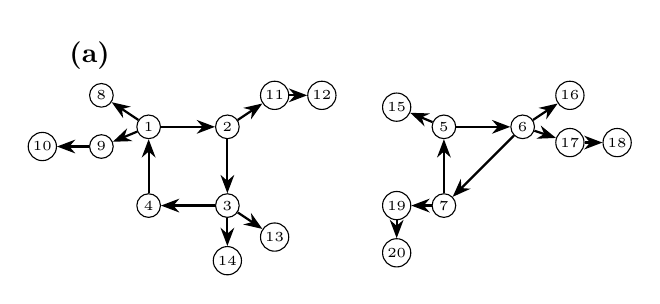
\begin{tikzpicture}[scale=0.5,
    every node/.style={circle, draw, minimum size=0.3cm, font=\tiny, inner sep=1pt},
    arrow/.style={-{Stealth}, thick},
    node distance=2.0cm
]
%% ============================================================
%% FIRST STRUCTURE: 4-loop (nodes 1,2,3,4) on a square + trees
%% ============================================================
\node (1) at (0,0)   {$1$};
\node (2) at (2,0)   {$2$};
\node (3) at (2,-2)  {$3$};
\node (4) at (0,-2)  {$4$};
\draw[arrow] (1) -- (2);
\draw[arrow] (2) -- (3);
\draw[arrow] (3) -- (4);
\draw[arrow] (4) -- (1);
\node (T1a) at (-1.2,  0.8) {$8$};
\node (T1b) at (-1.2, -0.5) {$9$};
\node (T1c) at (-2.7, -0.5) {$10$};
\draw[arrow] (1) -- (T1a);
\draw[arrow] (1) -- (T1b);
\draw[arrow] (T1b) -- (T1c);
\node (T2a) at (3.2,  0.8) {$11$};
\node (T2b) at (4.4,  0.8) {$12$};
\draw[arrow] (2) -- (T2a);
\draw[arrow] (T2a) -- (T2b);
\node (T3a) at (3.2, -2.8) {$13$};
\node (T3b) at (2.0, -3.4) {$14$};
\draw[arrow] (3) -- (T3a);
\draw[arrow] (3) -- (T3b);
%% ============================================================
%% SECOND STRUCTURE: 3-loop (nodes 5,6,7) shifted right + trees
%% ============================================================
\begin{scope}[xshift=7.5cm]
\node (5) at (0,0)   {$5$};
\node (6) at (2,0)   {$6$};
\node (8) at (0,-2)  {$7$};
\draw[arrow] (5) -- (6);
\draw[arrow] (6) -- (8);
\draw[arrow] (8) -- (5);
\node (S1a) at (-1.2,  0.5) {$15$};
\draw[arrow] (5) -- (S1a);
\node (S2a) at (3.2,  0.8)  {$16$};
\node (S2b) at (3.2, -0.4)  {$17$};
\node (S2c) at (4.4, -0.4)  {$18$};
\draw[arrow] (6) -- (S2a);
\draw[arrow] (6) -- (S2b);
\draw[arrow] (S2b) -- (S2c);
\node (S3a) at (-1.2, -2.0) {$19$};
\node (S3b) at (-1.2, -3.2) {$20$};
\draw[arrow] (8) -- (S3a);
\draw[arrow] (S3a) -- (S3b);
\end{scope}
%% Label (a)
\node[draw=none, font=\normalsize\bfseries] at (-1.5, 1.8) {(a)};
\end{tikzpicture}
\vspace{1.0em}
%% ============================================================
%% SUBFIGURE (b): Permutation diagram
%% ============================================================
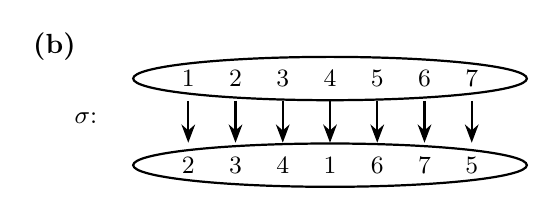
\begin{tikzpicture}[
    scale=0.5,
    pnode/.style={draw=none, font=\small, inner sep=2pt},
    parrow/.style={-{Stealth}, thick, shorten >=3pt, shorten <=3pt}
]
%% Label (b)
\node[pnode, font=\normalsize\bfseries] at (-7.0, 0.8) {(b)};
% --- Draw two ovals ---
\draw[thick] (0,0) ellipse (5.0cm and 0.55cm);
\draw[thick] (0,-2.2) ellipse (5.0cm and 0.55cm);
% --- Row labels ---
\node[pnode] at (-6.2, -1)    {$\sigma$:};
% --- Top row: 1 through 7, plain numbers ---
\foreach \i/\x in {1/-3.6, 2/-2.4, 3/-1.2, 4/0.0, 5/1.2, 6/2.4, 7/3.6} {
    \node[pnode] (top\i) at (\x, 0) {$\i$};
}
% --- Bottom row: sigma(i) values ---
\foreach \i/\x/\lbl in {1/-3.6/2, 2/-2.4/3, 3/-1.2/4, 4/0.0/1, 5/1.2/6, 6/2.4/7, 7/3.6/5} {
    \node[pnode] (bot\i) at (\x, -2.2) {$\lbl$};
}
% --- Arrows from top to bottom ---
\foreach \i in {1,2,3,4,5,6,7} {
    \draw[parrow] (top\i) -- (bot\i);
}
\end{tikzpicture}
\caption{(a)~Two disjoint $K=1$ Boolean network components, each consisting of
a loop of relevant nodes (numbered $1$--$4$ and $5$--$7$) with trees of
non-relevant nodes branching out. (b)~The corresponding permutation $\sigma$
on the relevant nodes, consisting of loops $(1\;2\;3\;4)$ and $(5\;6\;7)$:
the top row lists each node and the arrow indicates its image under $\sigma$.}
\label{fig:k1networks}
\end{figure}

Let $m$ denote the number of relevant nodes. Within the subnetwork induced by these nodes, every node has exactly one incoming and one outgoing edge. Thus, this subnetwork is naturally identified with a permutation $\sigma\in S_m$. For example, the relevant subnetwork in Fig.~\ref{fig:k1networks}a consists of a $4$-loop and a $3$-loop, corresponding to the permutation $(1\;2\;3\;4)(5\;6\;7)\in S_7$. The order of this permutation is the least common multiple of its cycle lengths, namely $\mathrm{ord}(\sigma)=\mathrm{lcm}(4,3)=12$.

It is known that every attractor length divides twice the least common multiple of the loop lengths, and, in particular cases (e.g., when all loops are positive), divides the least common multiple itself~\cite{Drosselcriticalk1network,flybjergexact}. Since the loop lengths are exactly the cycle lengths of the induced permutation, these results can be restated entirely in permutation-theoretic language: every attractor length in a critical $K=1$ network divides $2\,\mathrm{ord}(\sigma)$. 

The order of the induced permutation also determines the mean attractor length
and the number of attractors. In a critical $K=1$ network, the attractor states
are in one-to-one correspondence with the configurations of the $m$ relevant
nodes; there are therefore exactly $2^m$ of them, and the mean attractor length
is
\begin{equation}\label{eq:expected_length}
  \bar{A}=\frac{2^m}{c},
\end{equation}
where $c$ is the total number of attractors. Since every attractor has length
at most $2\,\mathrm{ord}(\sigma)$,
\begin{equation}
  \bar A\le 2\,\mathrm{ord}(\sigma),
\end{equation}
and in Theorem~\ref{thm:mean_att_len} in the appendix we establish the lower bound
\begin{equation}
  \frac{\mathrm{ord}(\sigma)}{4}\le\bar A.
\end{equation}
Thus $\bar A$ and $\mathrm{ord}(\sigma)$ differ by at most a constant factor, so
the asymptotic scaling of $\bar A$ is set by that of $\mathrm{ord}(\sigma)$.
Equivalently, the number of attractors satisfies
\begin{equation}
  \frac{2^{m-1}}{\mathrm{ord}(\sigma)}\le c\le\frac{2^{m+2}}{\mathrm{ord}(\sigma)},
\end{equation}
so up to a constant factor $c\sim 2^m/\mathrm{ord}(\sigma)$. Therefore,
questions about the long-term dynamics are naturally reformulated as questions
about the induced permutation.

This reformulation is the central conceptual advance underlying our analysis. Rather than studying long-term dynamics directly as a property of Boolean networks, we instead study the induced permutation. Different aspects of the dynamics are thereby recast as questions about different permutation-theoretic invariants. More generally, this viewpoint establishes a bridge between Boolean-network dynamics and permutation theory, opening the possibility of characterizing a broad range of dynamical properties using the rich algebraic, combinatorial, and probabilistic theory of permutations.


\section*{Typical versus extremal maximum attractor lengths}
Since attractor lengths are governed by permutation order, classical results on the order of random permutations immediately yield asymptotic bounds for attractor lengths in random Boolean networks. In a celebrated series of papers, Erd\H{o}s and Tur\'an~\cite{ErdosTuran1965,ErdosTuran1967a,ErdosTuran1967b,ErdosTuran1968} 
studied the distribution of the order of a uniformly random permutation 
$\sigma\in S_m$.
In particular, they showed that $\sigma$ satisfies
\begin{equation}
  P\!\left(\mathrm{ord}(\sigma)\le \exp\!\left(\frac{1+\epsilon}{2}\ln^2 m\right)\right) > 1-\delta
  \label{eq:erdos_turan}
\end{equation}
for any $\epsilon,\delta>0$ and all sufficiently large $m$~\cite{ErdosTuran1965}.
In other words, a typical random permutation has sub-exponential order. Since the attractor lengths are bounded by $2\,\mathrm{ord}(\sigma)$, and since the number of relevant nodes satisfies $m\le N$, the maximum attractor length $\ell_{\max}$ satisfies
\begin{equation}
  P\!\left(\ell_{\max} \le 2\exp\!\left(\frac{1+\epsilon}{2}\ln^2 N\right)\right) > 1-\delta
  \label{eq:period_bound_N}
\end{equation}
for sufficiently large $N$. Thus, Erd\H{o}s and Tur\'an's theorem immediately implies that almost all critical $K=1$ Boolean networks have sub-exponential maximum attractor lengths. By contrast, Landau~\cite{Landau1903} showed that 
\begin{equation}
    \max_{\sigma\in S_m}\log\mathrm{ord}(\sigma)\sim\sqrt{m\ln m},
\end{equation}
so there exist networks whose maximum attractor length grows as $\Theta(\exp[\sqrt{N\ln N}])$. Thus, the permutation formulation reveals a striking dichotomy: typical critical $K=1$ networks have sub-exponential maximum attractor lengths, whereas extremal networks attain exponentially larger ones.


\section*{Scaling of mean attractor length.}


Goh and Schmutz~\cite{schmutz} proved that
\begin{equation}
\log\mathbb E[\mathrm{ord} (\sigma)] = c\sqrt{\frac{m}{\ln m}}(1+o(1)),
\end{equation}
where $c\approx2.99047$. Since $\ln(m)$ grows slower than any polynomial power,
\begin{equation}
\log\mathbb E[\mathrm{ord} (\sigma)] = m^{1/2+o(1)}.
\end{equation}

Therefore, the mean attractor length of networks with $m$ relevant nodes scales as $\exp[m^{1/2+o(1)}]$. To obtain the expected mean attractor length over all critical $K=1$ networks with $N$ nodes, it remains only to average over the distribution of the number of relevant nodes. By~\cite{finkexponential,drosselreview},
\begin{equation}
P(m)\sim\frac{m}{N}\exp\!\left(-\frac{m^2}{2N}\right),
  \label{eq:Pm}
\end{equation}
so
\begin{equation}
  \label{eq:sum}
\mathbb E[\bar A] \sim \sum_{m=0}^{\infty} \frac{m}{N} 
\exp\!\left(-m^2/2N\right) 
\exp\!\left(m^{1/2+o(1)}\right).
\end{equation}

Setting $m=\sqrt N\,x$ and applying Laplace's method (see Lemma~\ref{lemma:asymptotics}) yields
\begin{equation}\label{eq:full_asymptotic}
\mathbb E[\bar A]
=
\exp\!\left(N^{1/3+o(1)}\right).
\end{equation}

Thus, although a typical critical $K=1$ network possesses sub-exponential
maximum attractor length, the expected mean attractor length is dominated by
rare networks whose exceptionally large permutation order gives rise to much
longer attractors.

\section*{Discussion.}
We have shown that the scaling of attractor lengths in
critical $K=1$ Boolean networks is fundamentally governed by the order of the permutation induced by the network's feedback loops. More broadly, we identified the induced permutation as the natural mathematical object underlying long-term network dynamics and reduces questions about these dynamics, such as attractor lengths, to questions in the theory of random permutations. Combining classical results of Erd\H{o}s and Tur\'an~\cite{ErdosTuran1965}, Landau's theorem~\cite{Landau1903}, and Goh and Schmutz's asymptotics for the expected permutation order~\cite{schmutz}, we obtain a complete asymptotic picture: almost all networks have sub-exponential maximum attractor lengths of order $\exp[O(\ln^2 N)]$, whereas rare extremal networks attain lengths as large as $\exp[\Theta(\sqrt{N\ln N})]$. Averaging over all network realizations then yields an expected mean attractor length of $\exp[N^{1/3+o(1)}]$, demonstrating that expectation values are dominated by rare networks with exceptionally large permutation order. Beyond these leading-order asymptotics, our approach also provides exact, albeit algebraically involved, finite-$N$ expressions for the mean attractor length (see Eq.~\ref{eq:ratio} in the appendix).

This distinction between typical and average behavior has important practical consequences. Because the distribution of attractor lengths is highly right-skewed, simulations that sample typical trajectories systematically underestimate the mean attractor length and therefore cannot reliably estimate expected dynamical quantities~\cite{finkexponential}. Understanding the full distribution of attractor lengths, rather than only its extreme and average behavior, therefore remains an important open problem.

Our analysis uses only the first layer of a much richer theory of random permutations. More recent results on the distribution of permutation order, refined asymptotics for $\log\mathrm{ord}(\sigma)$~\cite{ford2021cycle}, suggest that much more precise descriptions of attractor-length distributions should be obtainable. More broadly, the induced permutation provides a unifying framework extending beyond attractor lengths. Different dynamical quantities, including the number of attractors, basin-size statistics, and measures of dynamical entropy, depend on different arithmetic invariants of the same permutation, making them natural targets for the methods of algebraic combinatorics and probabilistic number theory.

Finally, the permutation-theoretic viewpoint may extend beyond the $K=1$ setting considered here. In critical $K=2$ Boolean networks, the dynamically relevant core reduces asymptotically to an effective $K=1$ structure~\cite{drosselreview}, suggesting that permutation-based methods may provide a route toward resolving the long-standing problem of attractor statistics in critical Boolean networks with higher connectivity.


\section*{Acknowledgments}
The authors thank Maria Siskaki for useful comments and
suggestions. 



\section*{Appendix}
This appendix contains a theorem together with its proof. The proof makes use of two lemmas that we state and prove after the theorem. Additionally, there is a lemma that details the computation of the asymptotic for the mean attractor length.
\\
\begin{theorem}\label{thm:mean_att_len}
    Suppose a critical $K=1$ network has mean attractor length $\bar{A}$ and permutation $\sigma$, then
\begin{equation}
  \frac{\bar{A}}{\mathrm{ord}(\sigma)}
  \;\ge\;
  \frac{1}{4}.
\end{equation}   
\end{theorem}

 





\begin{proof}
    

We proceed by a sequence of reductions.
We first show that for any Boolean network $F$ with at least one 
negative feedback loop, the network $F_+$ obtained by replacing all 
inhibitory edges with activating edges satisfies $\bar{A}(F_+) \le 
\bar{A}(F)$. Since $F$ and $F_+$ share the same underlying directed 
graph, they induce the same permutation $\sigma$, and therefore
$\bar{A}(F_+)/\mathrm{ord}(\sigma) \le \bar{A}(F)/\mathrm{ord}(\sigma)$,
so it suffices to prove the lower bound for networks consisting 
entirely of positive feedback loops. Within this class, we then show that 
$\bar{A}/\mathrm{ord}(\sigma)$ is minimized when every 
non-trivial (length $>1$) feedback loop has a prime-power 
length, so it suffices to consider networks of this form. Finally, we show that for any such network 
$\bar{A}/\mathrm{ord}(\sigma) \ge 1/4$, which establishes the theorem.


\paragraph{Step 1: Reduction to positive loops}
Let $F$ be a critical $K=1$ Boolean network containing at least one 
component whose long-term dynamics are governed by a negative feedback 
loop of length $n$; we denote this component $\bar{\mathbb{C}}_n$. 
Let $F'$ be the network obtained from $F$ by replacing all inhibitory 
edges in $\bar{\mathbb{C}}_n$ with activating edges, leaving all 
other update functions unchanged. We now show that $\bar{A}(F') \le 
\bar{A}(F)$. Applying this iteratively yields a network $F_+$ consisting 
entirely of components with positive feedback loops, satisfying 
$\bar{A}(F_+) \le \bar{A}(F)$ and 
$\mathrm{ord}(\sigma_{F_+}) = \mathrm{ord}(\sigma_F)$, so it 
suffices to prove the lower bound for $F_+$.

Recall from Eq.~\eqref{eq:expected_length} that $\bar{A} = 2^m/c$,
where $m$ is the total number of relevant nodes across all components 
and $c$ is the number of attractors. It therefore suffices to show 
that $c(F') \ge c(F)$. Writing $F = G \cup \bar{\mathbb{C}}_n$, 
where $G$ is the remainder of the network, the total number of 
attractors of $F$ is
\begin{equation}
  c(F) = \sum_{P} g(P)\sum_{\ell} \bar{c}(\ell)\,\gcd(\ell,P),
  \label{eq:attractors_F}
\end{equation}
where $g(P)$ is the number of attractors of length $P$ in $G$, and 
$\bar{c}(\ell)$ is the number of limit cycles of length $\ell$ 
determined by the negative feedback loop of length $n$ in 
$\bar{\mathbb{C}}_n$~\cite{demongeot2010number,Golomb2017}:
\begin{equation}\label{eq:negative_circuit}
\bar{c}(\ell) = \begin{cases}
\dfrac{1}{\ell}\displaystyle\sum_{\substack{d\mid \ell/2 \\ 
n/d \text{ odd}}}\mu(d)\cdot 2^{\ell/(2d)} 
& \substack{\text{if } \ell \text{ even, } \tfrac{\ell}{2} \mid n, \\
\text{ and } \tfrac{2n}{\ell} \text{ odd,}}\\[10pt]
0 & \text{otherwise.}
\end{cases}
\end{equation}
Since $F' = G \cup \mathbb{C}_n$ differs from $F$ only in that all 
inhibitory edges within $\bar{\mathbb{C}}_n$ have been replaced by 
activating edges, the number of attractors of $F'$ is
\begin{equation}
  c(F') = \sum_{P} g(P)\sum_{\ell} c(\ell)\,\gcd(\ell,P),
  \label{eq:attractors_Fprime}
\end{equation}
where $c(\ell)$ is the number of limit cycles of length $\ell$ 
determined by the positive feedback loop of length $n$ in 
$\mathbb{C}_n$~\cite{demongeot2010number,Golomb2017}:
\begin{equation}\label{eq:positive_circuit}
c(\ell) = \begin{cases}
\dfrac{1}{\ell}\displaystyle\sum_{d\mid \ell}
\mu\!\left(\frac{\ell}{d}\right)2^d
& \text{if } \ell \mid n,\\[10pt]
0 & \text{otherwise.}
\end{cases}
\end{equation}
Note that when $c(\ell)$ and $\bar{c}(\ell)$ are nonzero, their 
values depend only on $\ell$ and not on the loop length $n$.
Since $g(P) \ge 0$, it suffices to show that for all positive 
integers $n$ and $P$,
\begin{equation}
  \sum_{\ell} \bar{c}(\ell)\,\gcd(\ell,P) \;\le\; 
  \sum_{\ell} c(\ell)\,\gcd(\ell,P).
  \label{eq:reduction}
\end{equation}
Restricting the sums to the support of $c(\ell)$ and $\bar{c}(\ell)$ 
— namely divisors of $n$ — and substituting the explicit 
formulas~\eqref{eq:positive_circuit} and~\eqref{eq:negative_circuit}, 
Eq.~\eqref{eq:reduction} reduces to showing
\begin{equation}
  \sum_{\substack{q\mid n\\q\text{ odd}}}
  \bar{c}\!\left(\tfrac{2n}{q}\right)
  \left(\tfrac{2n}{q},P\right)
  \;\le\;
  \sum_{d\mid n} c(d)\,(d,P).
  \label{eq:neg_vs_pos}
\end{equation}
This follows from Lemma~\ref{lemma:positivereduction}
below, which concludes Step~1.

\paragraph{Step 2: Reduction to prime-power loop lengths}
By Step~1, it suffices to consider networks in which all feedback 
loops are positive, with non-trivial loop lengths $l_1,\ldots,l_k$. 
For such networks, the mean attractor length $\bar{A}$ depends only 
on the loop lengths $l_1,\ldots,l_k$ and not on the tree structure 
of the components, since the long-term dynamics are entirely 
determined by the relevant core. Therefore $\bar{A}/L$ is a 
function of the loop lengths alone, and it is meaningful to minimize 
over all possible choices of loop lengths. Since 
$\mathrm{ord}(\sigma) = L = \mathrm{lcm}(l_1,\ldots,l_k)$, the 
lower bound $\bar{A} \ge \mathrm{ord}(\sigma)/4$ is equivalent to 
$\bar{A}/L \ge 1/4$. Applying Burnside's lemma, 
the total number of attractors is
\begin{equation}
  c = \frac{1}{L}\sum_{j=0}^{L-1}\prod_{i=1}^{k} 
  2^{\gcd(j,\,l_i)},
  \label{eq:burnside_lemma}
\end{equation}
and since $\bar{A} = 2^{\sum_i l_i}/c$, we have
\begin{equation}
  \frac{\bar{A}}{L}
  \;=\;
  \frac{2^{\sum_i l_i}}{\sum_{j=0}^{L-1}\prod_{i=1}^{k} 
  2^{\gcd(j,\,l_i)}}.
  \label{eq:ratio}
\end{equation}
Note that loops of length $1$ contribute equally to the numerator 
and denominator of Eq.~\eqref{eq:ratio} and therefore do not affect 
$\bar{A}/L$, so it suffices to consider non-trivial loops only. We 
now show via two observations that the minimum of $\bar{A}/L$ over 
all choices of non-trivial loop lengths occurs when these lengths 
are distinct prime powers.

First, suppose one loop has length $l_1 = ab$ with $\gcd(a,b)=1$. 
Consider a new network $F'$ whose relevant core consists of two 
components with loops of lengths $a$ and $b$ respectively, together 
with the remaining loops $l_2,\ldots,l_k$ unchanged. Since the 
long-term dynamics depend only on the relevant core, the tree 
structure of the new components can be arbitrary. The nodes that 
were on the original loop of length $ab$ are accounted for by 
trivial loops of length $1$ in $F'$, which do not affect $\bar{A}/L$ 
as established above. Since $\gcd(a,b)=1$, we have 
$\mathrm{lcm}(a,b,l_2,\ldots,l_k) = \mathrm{lcm}(ab,l_2,\ldots,l_k) 
= L$, so the denominator $L$ is unchanged. We claim that
\begin{equation}
  \frac{\bar{A}(F')}{L} \;\le\; \frac{\bar{A}(F)}{L},
  \label{eq:coprime_split}
\end{equation}
i.e.\ splitting a composite-length loop into coprime parts does 
not increase $\bar{A}/L$. This follows from the pointwise 
inequality
\begin{equation}
  \gcd(j,ab) \le \gcd(j,a) + \gcd(j,b) + ab - a - b - 1,
\end{equation}
which gives 
$2^{\gcd(j,ab)}\le 2^{\gcd(j,a)}\cdot 2^{\gcd(j,b)}\cdot 
2^{ab-a-b}$, and hence
\begin{align}
  &\sum_{j=0}^{L-1}\prod_{i=2}^k 2^{\gcd(j,l_i)}\cdot 
  2^{\gcd(j,ab)} \nonumber\\
  &\quad\le\;
  2^{ab-a-b}\sum_{j=0}^{L-1}\prod_{i=2}^k 
  2^{\gcd(j,l_i)}\cdot 2^{\gcd(j,a)}\cdot 2^{\gcd(j,b)}.
\end{align}
Eq.~\eqref{eq:coprime_split} follows from simple alebraic manifpulation.
Repeated application 
reduces to networks where every non-trivial loop length is a 
prime power.

Second, suppose the relevant core contains a loop of length $d$ 
such that $d$ divides $\mathrm{lcm}(l_2,\ldots,l_k)$, so that 
$L$ is unchanged by removing it. Consider the network $F''$ 
obtained by removing this loop from the relevant core (replacing 
it with  trivial loops of length $1$). The numerator of 
Eq.~\eqref{eq:ratio} loses a factor of $2^d$, while the 
denominator loses a factor of 
$\frac{1}{L}\sum_{j=0}^{L-1} 2^{\gcd(j,d)} \le 2^d$, 
since $\gcd(j,d) \le d$ for all $j$. Hence removing such a loop 
does not decrease $\bar{A}/L$, so the minimum is achieved for 
networks whose non-trivial loop lengths are distinct prime powers.

Combining these two observations, it suffices to prove 
$\bar{A}/L \ge 1/4$ for networks whose relevant core consists 
of loops of distinct prime-power lengths 
$p_1^{a_1},\ldots,p_r^{a_r}$ with distinct primes $p_i$.

\paragraph{Step 3: Lower bound for prime-power loop lengths}
For networks with distinct prime-power loop lengths 
$p_1^{a_1},\ldots,p_r^{a_r}$, the loop lengths are pairwise 
coprime, so $\gcd(j, p_i^{a_i})$ depends only on $j \bmod p_i^{a_i}$. 
Applying the Chinese Remainder Theorem to 
Eq.~\eqref{eq:burnside_lemma} therefore gives the factorization
\begin{equation}
  \frac{\bar{A}(p_1^{a_1},\ldots,p_r^{a_r})}{L}
  = \prod_{i=1}^r \frac{\bar{A}(p_i^{a_i})}{p_i^{a_i}}.
\end{equation}
For a single positive loop of prime-power length $p^a$, 
evaluating Eq.~\eqref{eq:ratio} explicitly gives
\begin{equation}
\frac{\bar{A}(p^a)}{p^a}
= \frac{2^{p^a}}{2^{p^a} + \sum_{j=1}^{a} p^{j-1}(p-1)\cdot 
2^{p^{a-j}}},
\label{eq:ratio_pk}
\end{equation}
which at $a=1$ reduces to
\begin{equation}
\frac{\bar{A}(p)}{p}
= \frac{2^p}{2^p + 2(p-1)}.
\label{eq:ratio_prime}
\end{equation}
By Lemma~\ref{lemma:primepowers} below, $\bar{A}(p^a)/p^a \ge \bar{A}(p)/p$ for all 
$a \ge 1$, so combining with the factorization gives
\begin{align}
  \frac{\bar{A}}{L}
  &= \prod_{i=1}^r \frac{\bar{A}(p_i^{a_i})}{p_i^{a_i}}
  \;\ge\;
  \prod_{i=1}^r \frac{\bar{A}(p_i)}{p_i}
  \;\\&\ge\;
  \prod_{p\;\text{prime}} \frac{2^p}{2^p+2(p-1)}
  \;=:\; R_{\min},
\end{align}
where the last inequality holds since each factor is less than 
one, so extending the finite product to all primes can only 
decrease it. The infinite product $R_{\min}$ converges, and a 
numerical computation gives $R_{\min} \sim 0.32 > 1/4$, from which we conclude $\bar{A}/L \ge 1/4$, 
i.e.\ $\bar{A} \ge \mathrm{ord}(\sigma)/4$. 

\end{proof}

We now prove Lemma~\ref{lemma:positivereduction}, Lemma~\ref{lemma:primepowers} that were required in the proof of Theorem~\ref{thm:mean_att_len}. These two lemmas were formally verified using the Aristotle API~\cite{aristole}.
\begin{lemma}\label{lemma:positivereduction}
   With $c(\ell)$ and $\bar{c}(\ell)$ as in 
Eqs.~\eqref{eq:positive_circuit} and~\eqref{eq:negative_circuit}, 
the following identity holds for all positive integers $k$:
\begin{equation}
  \bar{c}(2k)\cdot 2k = \sum_{\substack{d\mid k\\\text{$k/d$ 
  a power of 2}}} d\cdot c(d).
  \label{eq:break2mcycles}
\end{equation} 
\end{lemma}


\begin{proof}
    

Since every state of a positive loop of length 
$n$ lies on an attractor, the total number of states in limit 
cycles satisfies~\cite{demongeot2010number}
\begin{equation}
  \sum_{d'\mid n} c(d')\,d' = 2^n.
  \label{eq:total_states}
\end{equation}
Substituting $n = k/d$ into Eq.~\eqref{eq:total_states} and 
inserting into the formula for $\bar{c}(2k)$ from 
Eq.~\eqref{eq:negative_circuit} gives
\begin{equation}
  \bar{c}(2k)\cdot 2k = \sum_{\substack{d\mid k \\ 
  k/d \text{ odd}}}\mu(d)\cdot \sum_{d'\mid(k/d)}c(d')\,d'.
\end{equation}
Exchanging the order of summation, the coefficient of $c(d')d'$ 
becomes $\sum_{\substack{e \mid (k/d') \\ k/(ed') \text{ odd}}} 
\mu(e)$, which equals $1$ if $k/d'$ is a power of $2$ and $0$ 
otherwise. This yields
\begin{equation}
  \bar{c}(2k)\cdot 2k = \sum_{\substack{d'\mid k\\ 
  k/d' \text{ a power of }2}} d'\cdot c(d'),
\end{equation}
which is the required equality. 
\end{proof}

\begin{lemma}\label{lemma:primepowers}
The ratio 
$\bar{A}(p^a)/p^a$ is minimized at $a=1$, i.e.\ for any prime 
$p$ and positive integer $a$,
\begin{equation}
  \frac{2^p}{2^p + 2(p-1)} \leq \frac{2^{p^a}}{2^{p^a} + 
  \sum_{j=1}^{a} p^{j-1}(p-1)\cdot 2^{p^{a-j}}}.
\end{equation}
\end{lemma}

\begin{proof}
    

Since all quantities are positive, both sides 
have the form $X/(X+Y)$ and cross-multiplying reduces the 
inequality to
\begin{equation}
  2^p\cdot\sum_{j=1}^{a} p^{j-1}(p-1)\cdot 2^{p^{a-j}} 
  \leq 2(p-1)\cdot 2^{p^a}.
\end{equation}
Factoring out $p-1 > 0$ reduces this to
\begin{equation}\label{eq:reduced_ineq}
  2^p\cdot\sum_{j=1}^{a} p^{j-1}\cdot 2^{p^{a-j}} \leq 2^{p^a+1},
\end{equation}
which we prove by induction on $a$. For $a=1$ both sides equal 
$2^p$, so equality holds. Assuming Eq.~\eqref{eq:reduced_ineq} 
at level $a$, the left-hand side at level $a+1$ is
\begin{align}
  2^p\sum_{j=1}^{a+1} p^{j-1}\cdot 2^{p^{a+1-j}}
  &= 2^p\cdot\left(2^{p^a} + p\cdot\sum_{j=1}^{a} 
  p^{j-1}\cdot 2^{p^{a-j}}\right) \nonumber\\
  &\leq 2^p\cdot\left(2^{p^a} + p\cdot 
  \frac{2^{p^a+1}}{2^p}\right) \nonumber\\
  &= 2^{p^a}\cdot\left(2^p + 2p\right),
\end{align}
where we used the inductive hypothesis in the second line. It 
therefore suffices to show that
\begin{equation}
  2^{p^{a+1}-p^a} \;\ge\; 2^{p-1}+p.
  \label{eq:suffices}
\end{equation}
Since $p^{a+1}-p^a = p^a(p-1) \ge p(p-1) \ge p$ for $p\ge 2$ 
and $a \ge 1$, we have $2^{p^{a+1}-p^a} \ge 2^p \ge 2\cdot 
2^{p-1} \ge 2^{p-1}+p$, where the last step uses $2^{p-1}\ge p$, 
which holds for all primes $p$.
\end{proof}

Finally, we prove the Lemma~\ref{lemma:asymptotics} required to compute the asymptotics of the mean attractor length.
\begin{lemma}\label{lemma:asymptotics}
    

The integral \begin{equation}
  I = \int_{0}^{\infty} x\,e^{\phi_N(x)}\,dx,
  \label{eq:substituted}
\end{equation}
where
\begin{equation}
  \phi_N(x) = -\frac{x^2}{2} + \left(Nx^2\right)^{1/4+o(1)},
  \label{eq:phase}
\end{equation}
satisfies 
\begin{equation}
  \log I = N^{1/3+o(1)}.
  \label{eq:full_asymptotic}
\end{equation}
\end{lemma}
\begin{proof}
Since $\phi_N(x)\to-\infty$ as $x\to\infty$, the integral is dominated by 
the unique maximum of $\phi_N$. Setting $\phi_N'(x_*)=0$ gives 
$x_* = N^{1/6+o(1)}$, at which
\begin{equation}
  \phi_N(x_*) = N^{1/3+o(1)}.
\end{equation}
Applying Laplace's method~\cite{debruijn1981asymptotic} and absorbing 
sub-exponential prefactors into the $o(1)$ exponent, we conclude
\begin{equation}
  \log I = N^{1/3+o(1)}.
  \label{eq:full_asymptotic}
\end{equation}
\end{proof}
















%%%%%%%%%%%%%%%%%%%%%%%%%%%%%%%%%%%%%%%%%%%%%%%
%% REFERENCES
%%%%%%%%%%%%%%%%%%%%%%%%%%%%%%%%%%%%%%%%%%%%%%%%
%\bibliographystyle{siam}
%\bibliographystyle{abbrv}
\bibliographystyle{unsrt}
% \bibliographystyle{ieeetr}
%\bibliographystyle{siamplain}

% Bibliography
\bibliography{references}





\end{document}




